%
\chapter{State of the art}%
Even though the focus in this research lies on a varying height robot model to use in planning and control, it is important to know recent work around humanoid robotics outside this area only, to understand what strategies are currently used in overall planning and control of bipeds. For these topics, a relatively more superficial evaluation is conducted and special attention is given to papers that were applied to Boston Dynamics' Atlas or NASA's Valkyrie at IHMC, as research is conducted and hopefully applied at this institute. Furthermore, walking and humanoid robot terminology is very extensive. A full in-depth study is performed on publications that address varying CoM height directly.

\section{Walking Terminology}
There are a variety of terms used in describing walking or locomotion, which can sometimes sound contradictive to each other. In this section the terminology in this report is determined, which is also widely used.
\subsection{Swing phase}
During the Swing Phase, the biped is only with one foot on the ground. The other foot is swinging through the air without ground contact, in the process of taking a step. The leg in contact with the ground is called the \textit{Stance Leg} and the leg taking a step is called the \textit{Swing Leg}. In a simplified walking model the Swing Phase with hybrid switching between legs is often the only phase considered. There exist also bipedal robots with only this phase, like ATRIAS from Oregon State University [REF REF]. This robot however, by the point-foot support with only a single leg per Swing Phase, has to keep stepping without interruption to stay stable.
\subsection{Transfer phase}
In more human like walking, next to the Swing Phase the Transfer Phase is considered, also called the Double Support Phase [REF REF]. This is the phase during walking where both feet are on the ground.

\section{\ac{LIP} models}
In modeling of walking, one of the most important assumptions is the modeling of the Stance Leg as a \ac{LIP}. In the \ac{2D} \ac{LIP} equations of motion
\begin{equation}
\ddot{x}=\frac{g}{l}x
\label{eq:LIPeom}
\end{equation}
where $l$ is the pendulum length and $x$ the Cartesian x-coordinate of the pendulum tip, the motion of the tip along the x-axis does not affect $l$. At any position $x$, a local straight pendulum is here considered, so this motion is on a constant height and $l=z_0$  holds. [SAY SOMETHING ABOUT INTUITIVELY NO HEIGHT ACCELERATION DESIRED].
\begin{figure}[h]
\centering
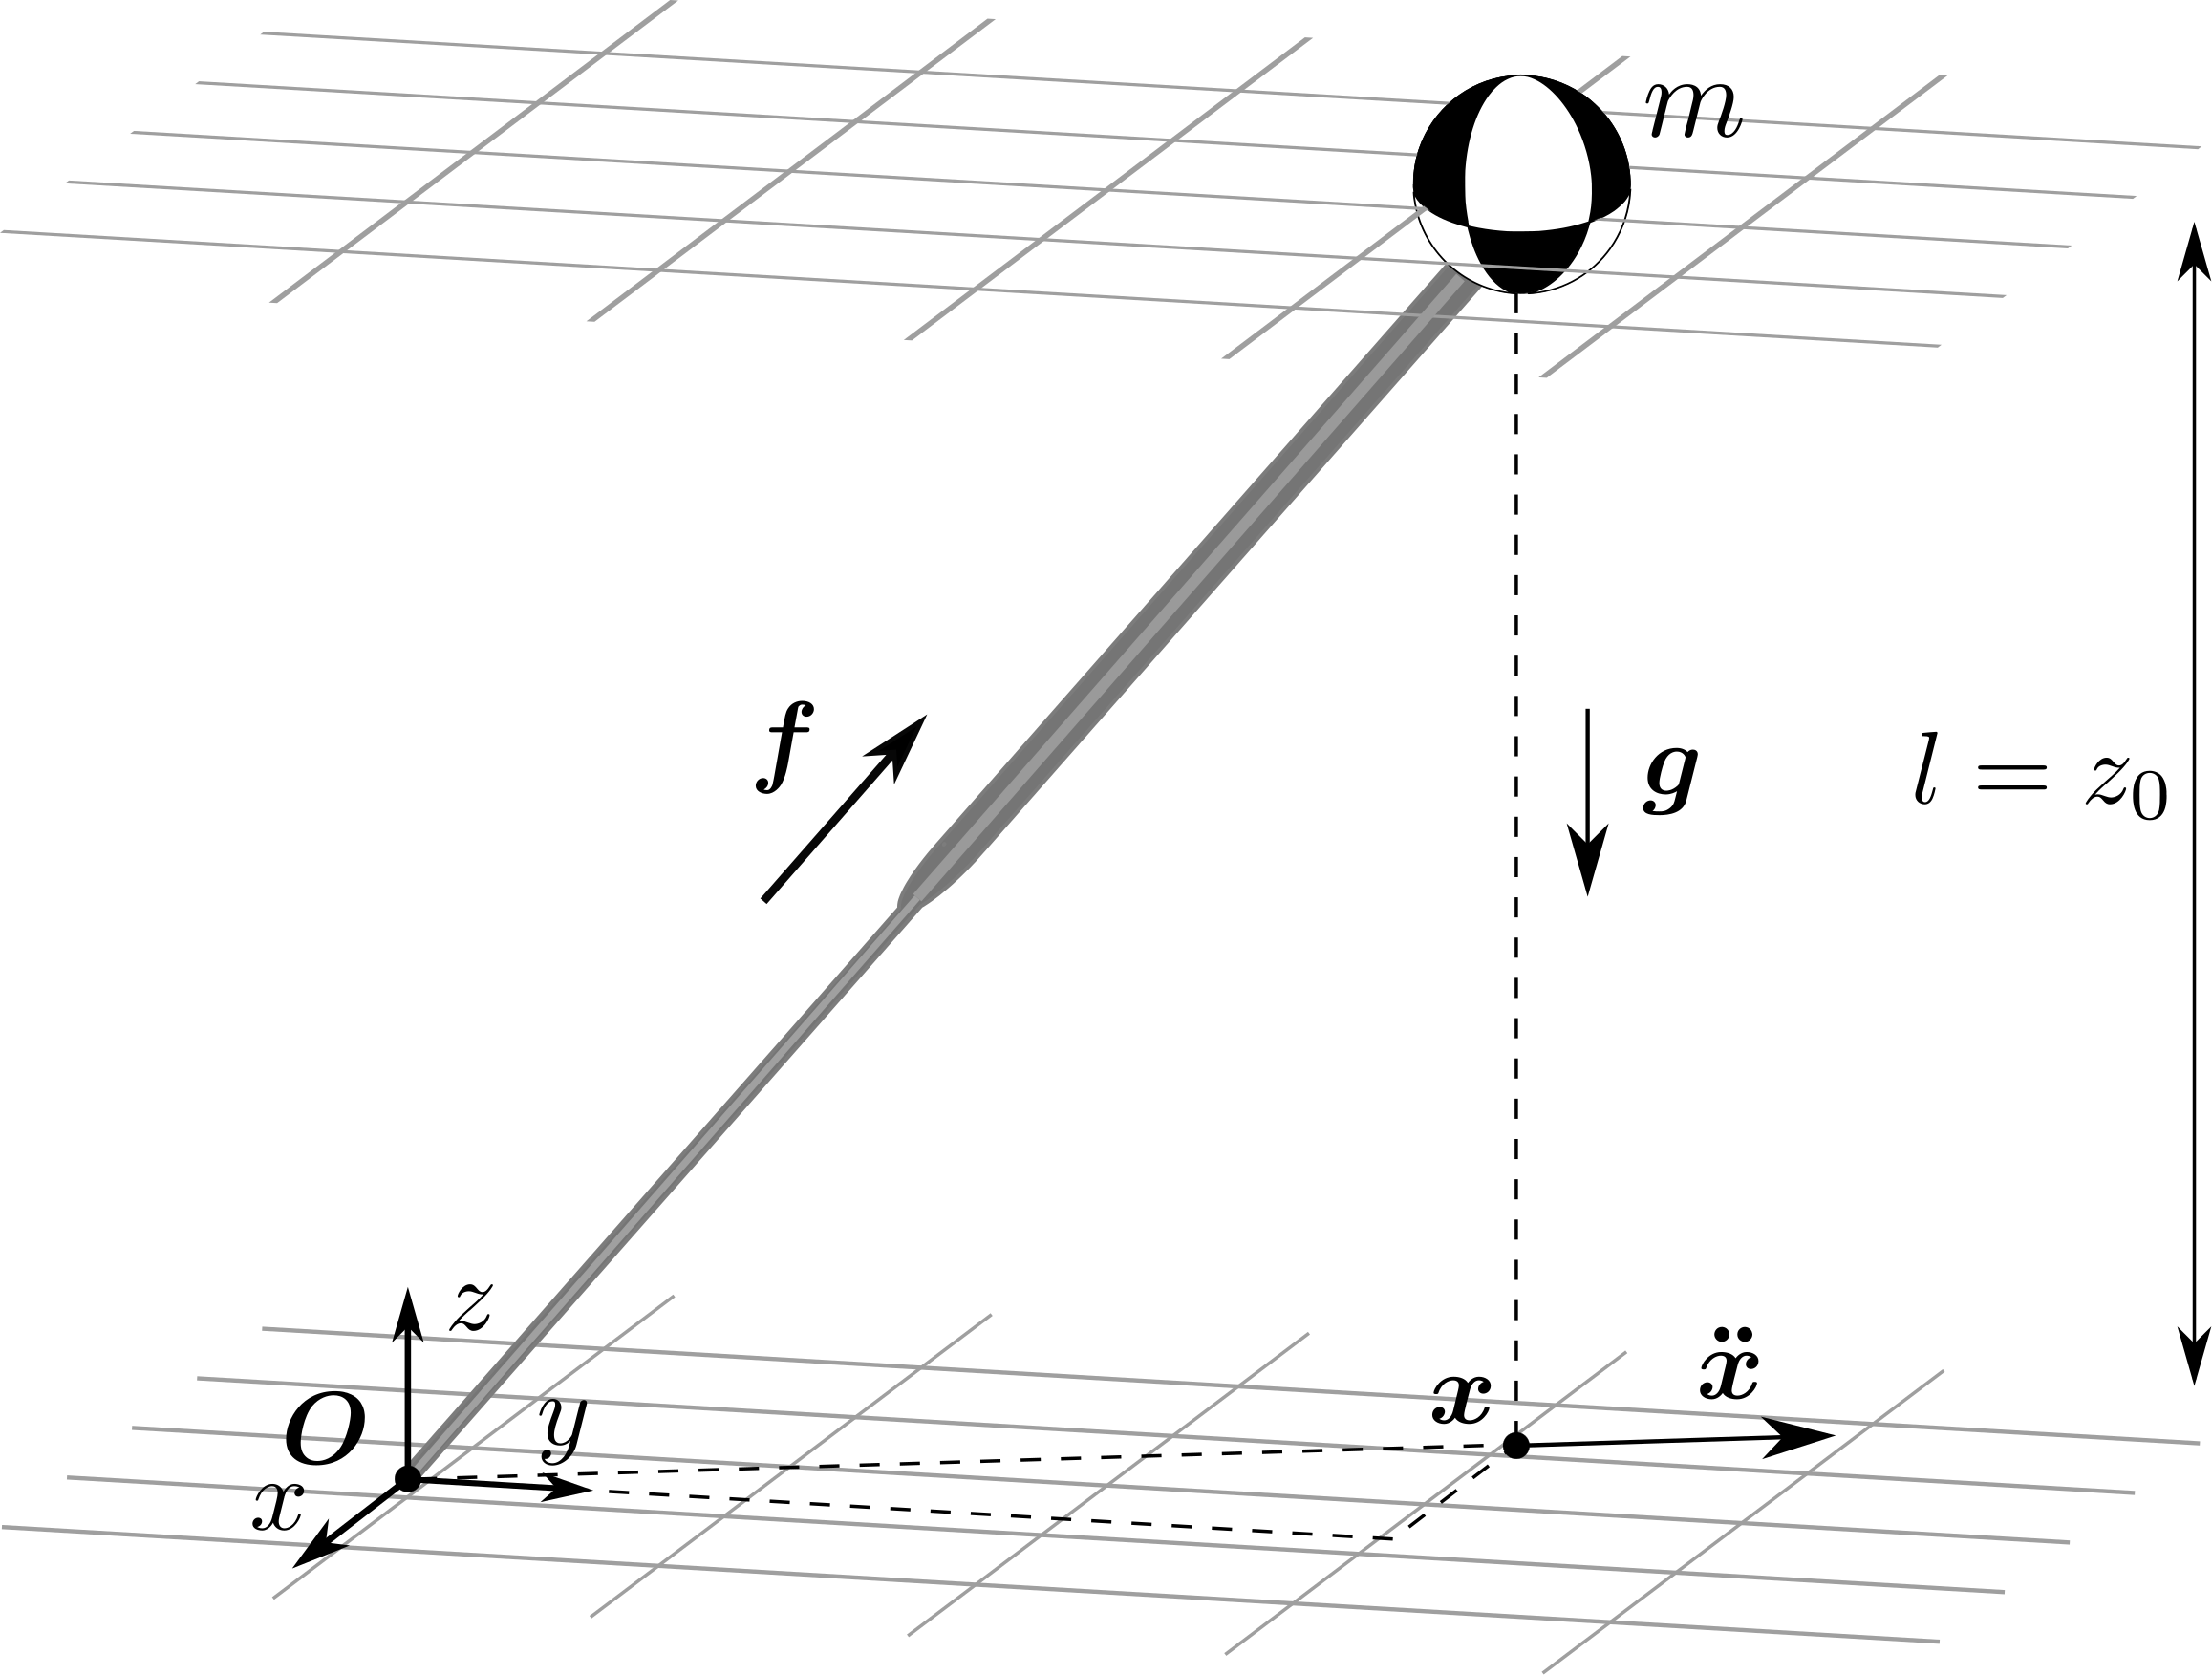
\includegraphics[width=0.5\textwidth]{STYLESTUFF/3DCoMwithoutfoot.png}
\caption{\ac{3D} motion of \ac{LIP} model}
\label{fig:3dlip}
\end{figure}
\subsection{Conservation of \ac{LIP} Orbital Energy}
\cite{kajita1992dynamic} had a crucial finding in an extended use of \ac{LIP} models. Because $F=ma$, $I=Fv$ and $E = Fs = \int Fv dt$, there can be reasoned that if one takes the time integral of the product of the second and the first derivative of a state, an expression for a normalized energy can be achieved: $\frac{E}{m}=\int av dt$. In the mentioned publication that same action is applied on Eq. \eqref{eq:LIPeom}:
\begin{equation}
\int (\ddot{x}-\frac{g}{l}x)\dot{x} dt = \frac{1}{2}\dot{x}^2-\frac{g}{2z_0}x +C
\label{eq:Elip}
\end{equation}
with $C$ the integration constant. The \ac{LIP} Orbital Energy is defined as $E_{LIP}=-C$. 
\subsection{The \ac{ICP}}
Although the finding of the \ac{LIP} Orbital Energy was very important for future robot motion modelling, more than a decade later \cite{pratt2006capture} introduced the Capture Point, also called the \acl{ICP}. Taking $E_{LIP}=0$ and taking the square root of Eq.  \eqref{eq:Elip} gives
\begin{equation}
x_{ICP}=\sqrt{ \frac{z_0}{g}\dot{x} }
\label{eq:cp}
\end{equation}
where $x_{ICP}$ is the \ac{ICP}, measured from the current pendulum tip position, based on the current tip velocity $\dot{x}$. This is the point where the velocity is driven to zero and the pendulum is upright. 
\section{Whole Robot Model}
\section{State Estimation}
\section{Humanoid Robot Terminology}
As the \ac{ICP} is a measure for the behavior of a bipedal robot, there exist plenty of terms and descriptions for specific virtual points and forces on and acting on the robot. In this section a short summary is given from the most popular jargon.
\subsection{The \ac{CoP}}
The larger feet of a human than those of a dog make him more capable of upright walking, due to an increase of controllability of the modeled-as-\ac{LIP} human. The ankles can apply a torque that virtually would move the base of the inverted pendulum, so that the linear acceleration on the \ac{CoM} as in Eq. \eqref{eq:LIPeom} and the capture point as in Eq. \eqref{eq:cp} change. The new virtual base is called the \ac{CoP}. By its definition, this point only lives within the foot polygon. [REF REF]
\begin{figure}[h]
\centering
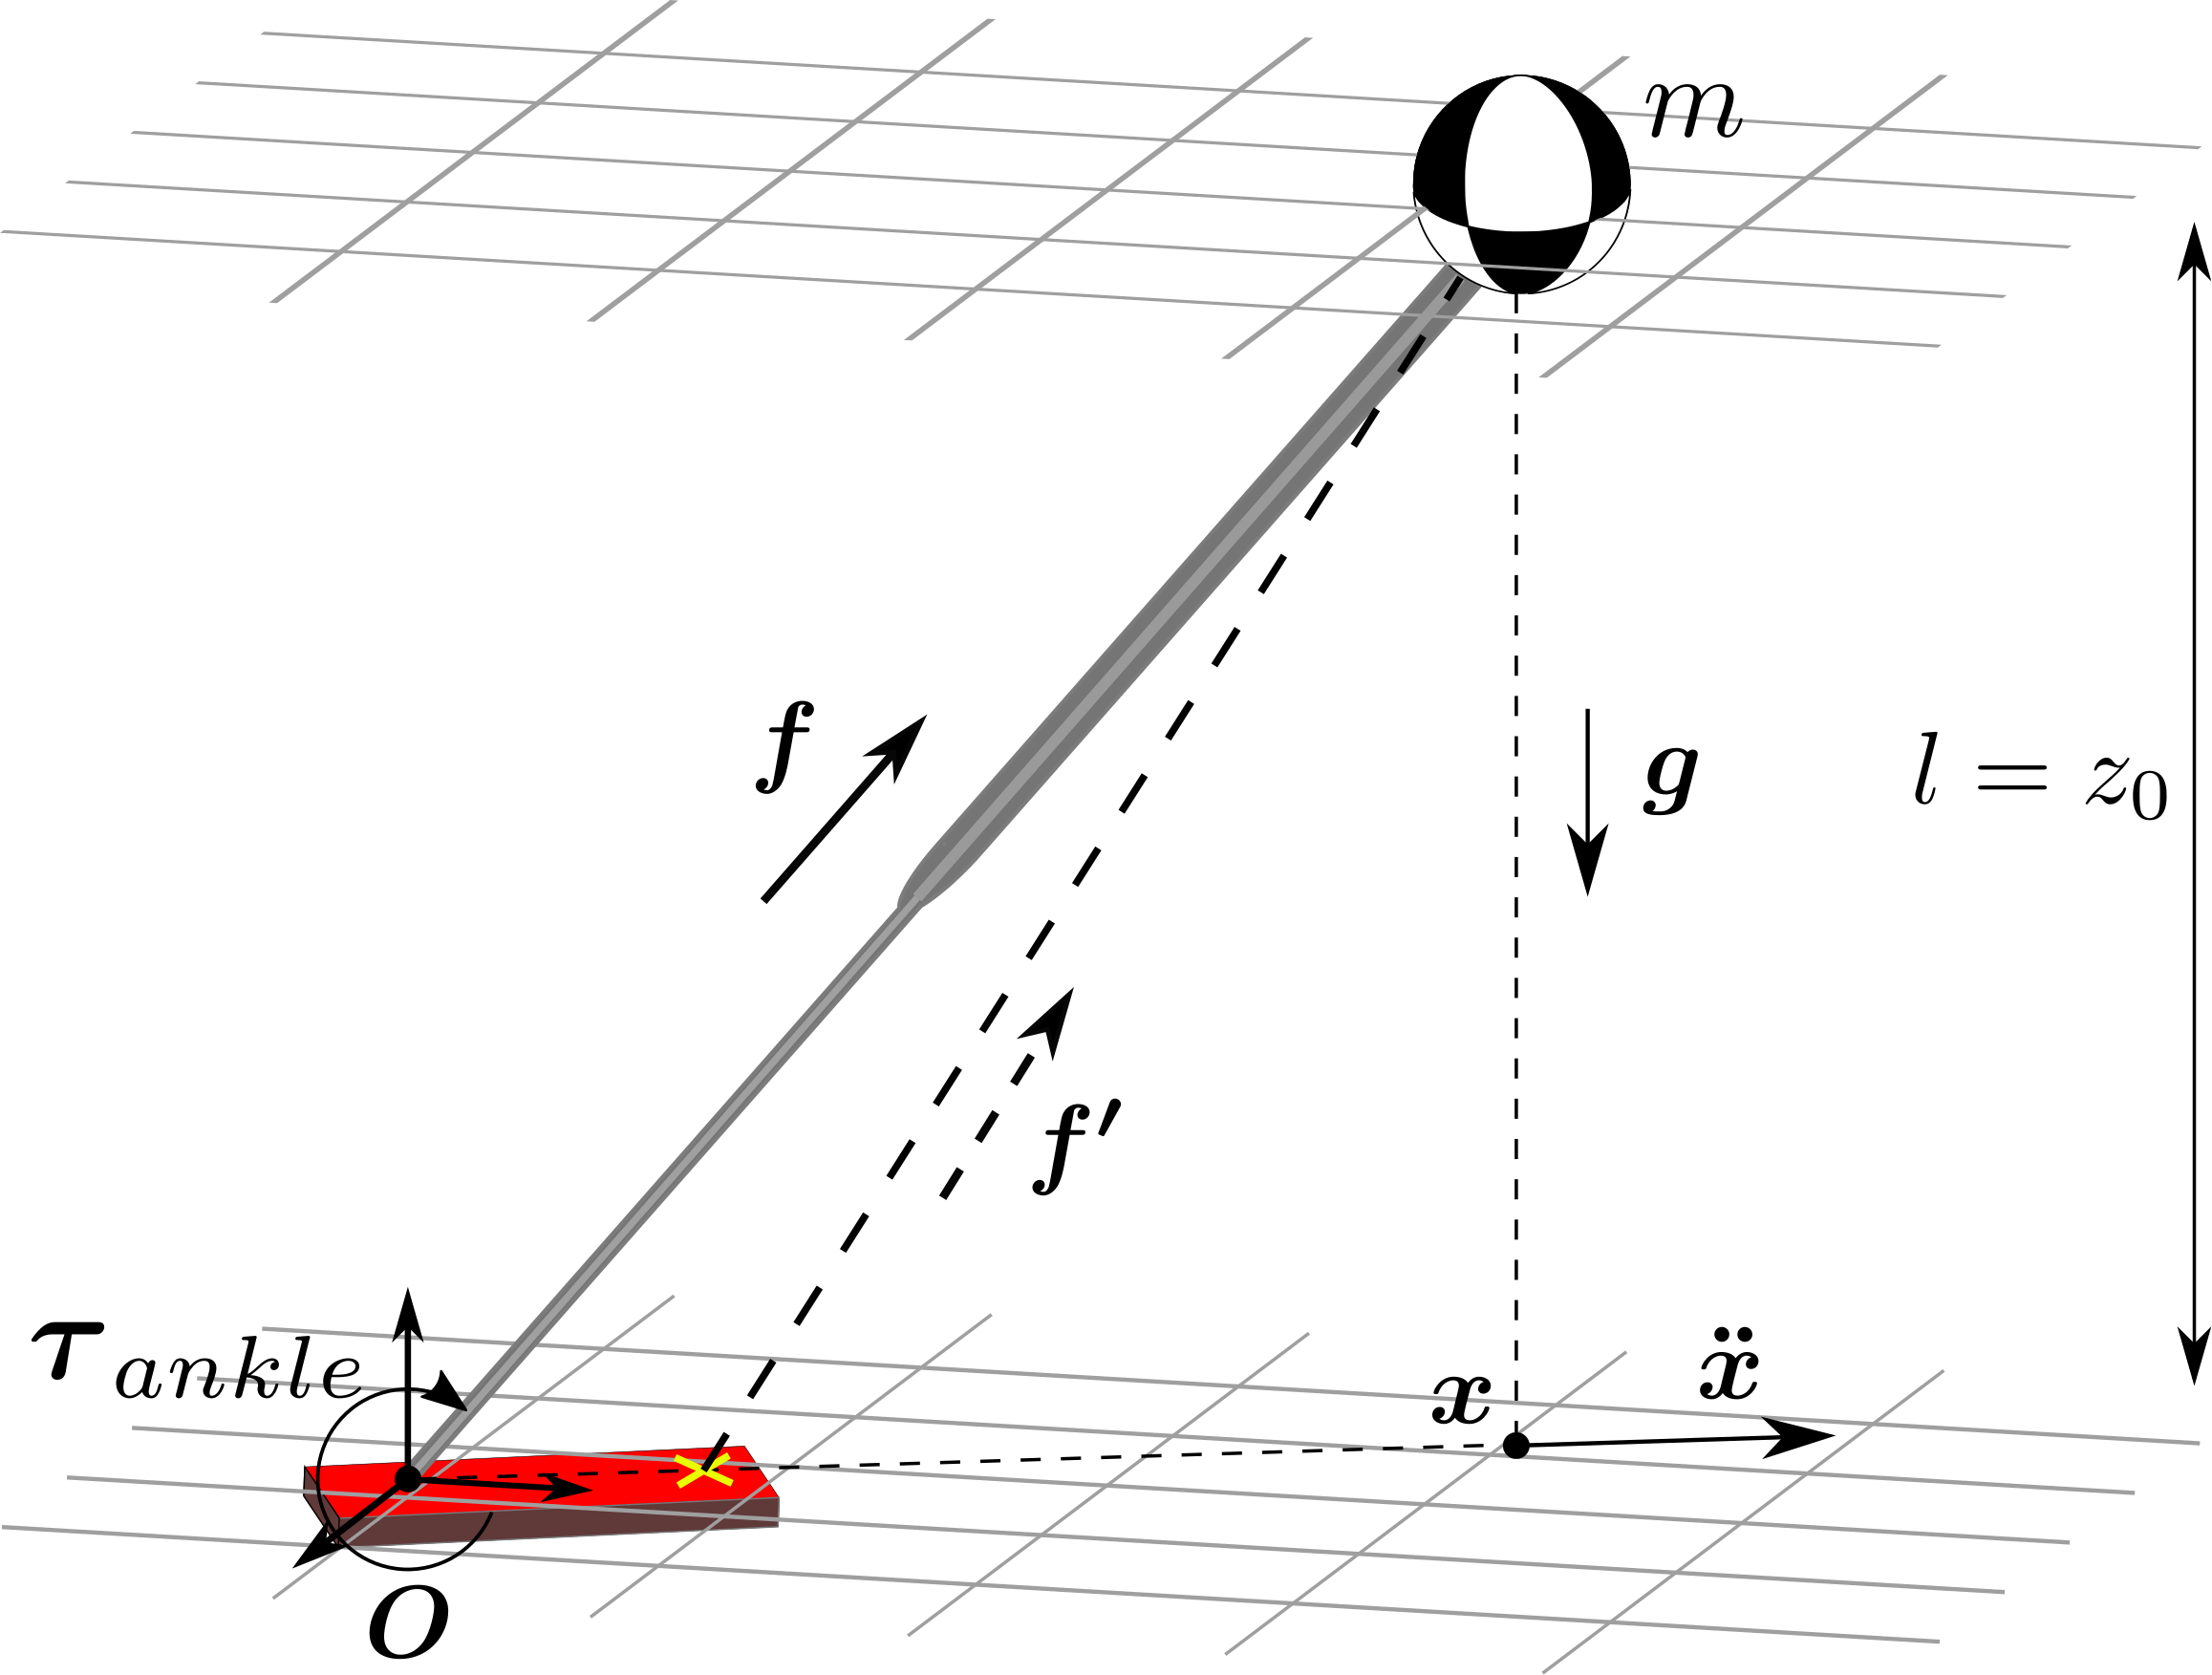
\includegraphics[width=0.5\textwidth]{STYLESTUFF/3DCoMwithfoot.png}
\caption{\ac{3D} motion of \ac{LIP} model with foot}
\label{fig:3dlipfoot}
\end{figure}
\subsection{The \ac{ZMP}}
The \ac{ZMP} coincides during stable walking with the \ac{CoP}, like described in \cite{vukobratovic2004zero}. The two points however are not equal in unstable or more complicated cases, like falling, running or walking over uneven terrain. How they differ is not further considered here.
\subsection{The \ac{CMP}}
The earlier mentioned points give sufficient measure for a \ac{LIP} model with point mass and finite sized feet. However, any angular momentum applied by the body does not affect those points. The \ac{CMP} takes angular momentum into account, which can be used as a measure and for control \cite{popovic2005ground}. This is defined as the point where a line passing through the \ac{CoM}, parallel to the ground reaction force intersects with the ground surface. The \ac{CMP} is defined as
\begin{eqnarray}
x_{CMP} = x_{ZMP} + \frac{\tau_y(\boldsymbol{r}_{CoM})}{F_{gr,z}}\\
y_{CMP} = y_{ZMP} - \frac{\tau_x(\boldsymbol{r}_{CoM})}{F_{gr,z}}
\end{eqnarray}
where $r_{CoM}$ is the location of the body \ac{CoM} and $F_{gr,z}$ is the ground reaction force in z-direction in Cartesian space. 
\begin{figure}[h]
\centering
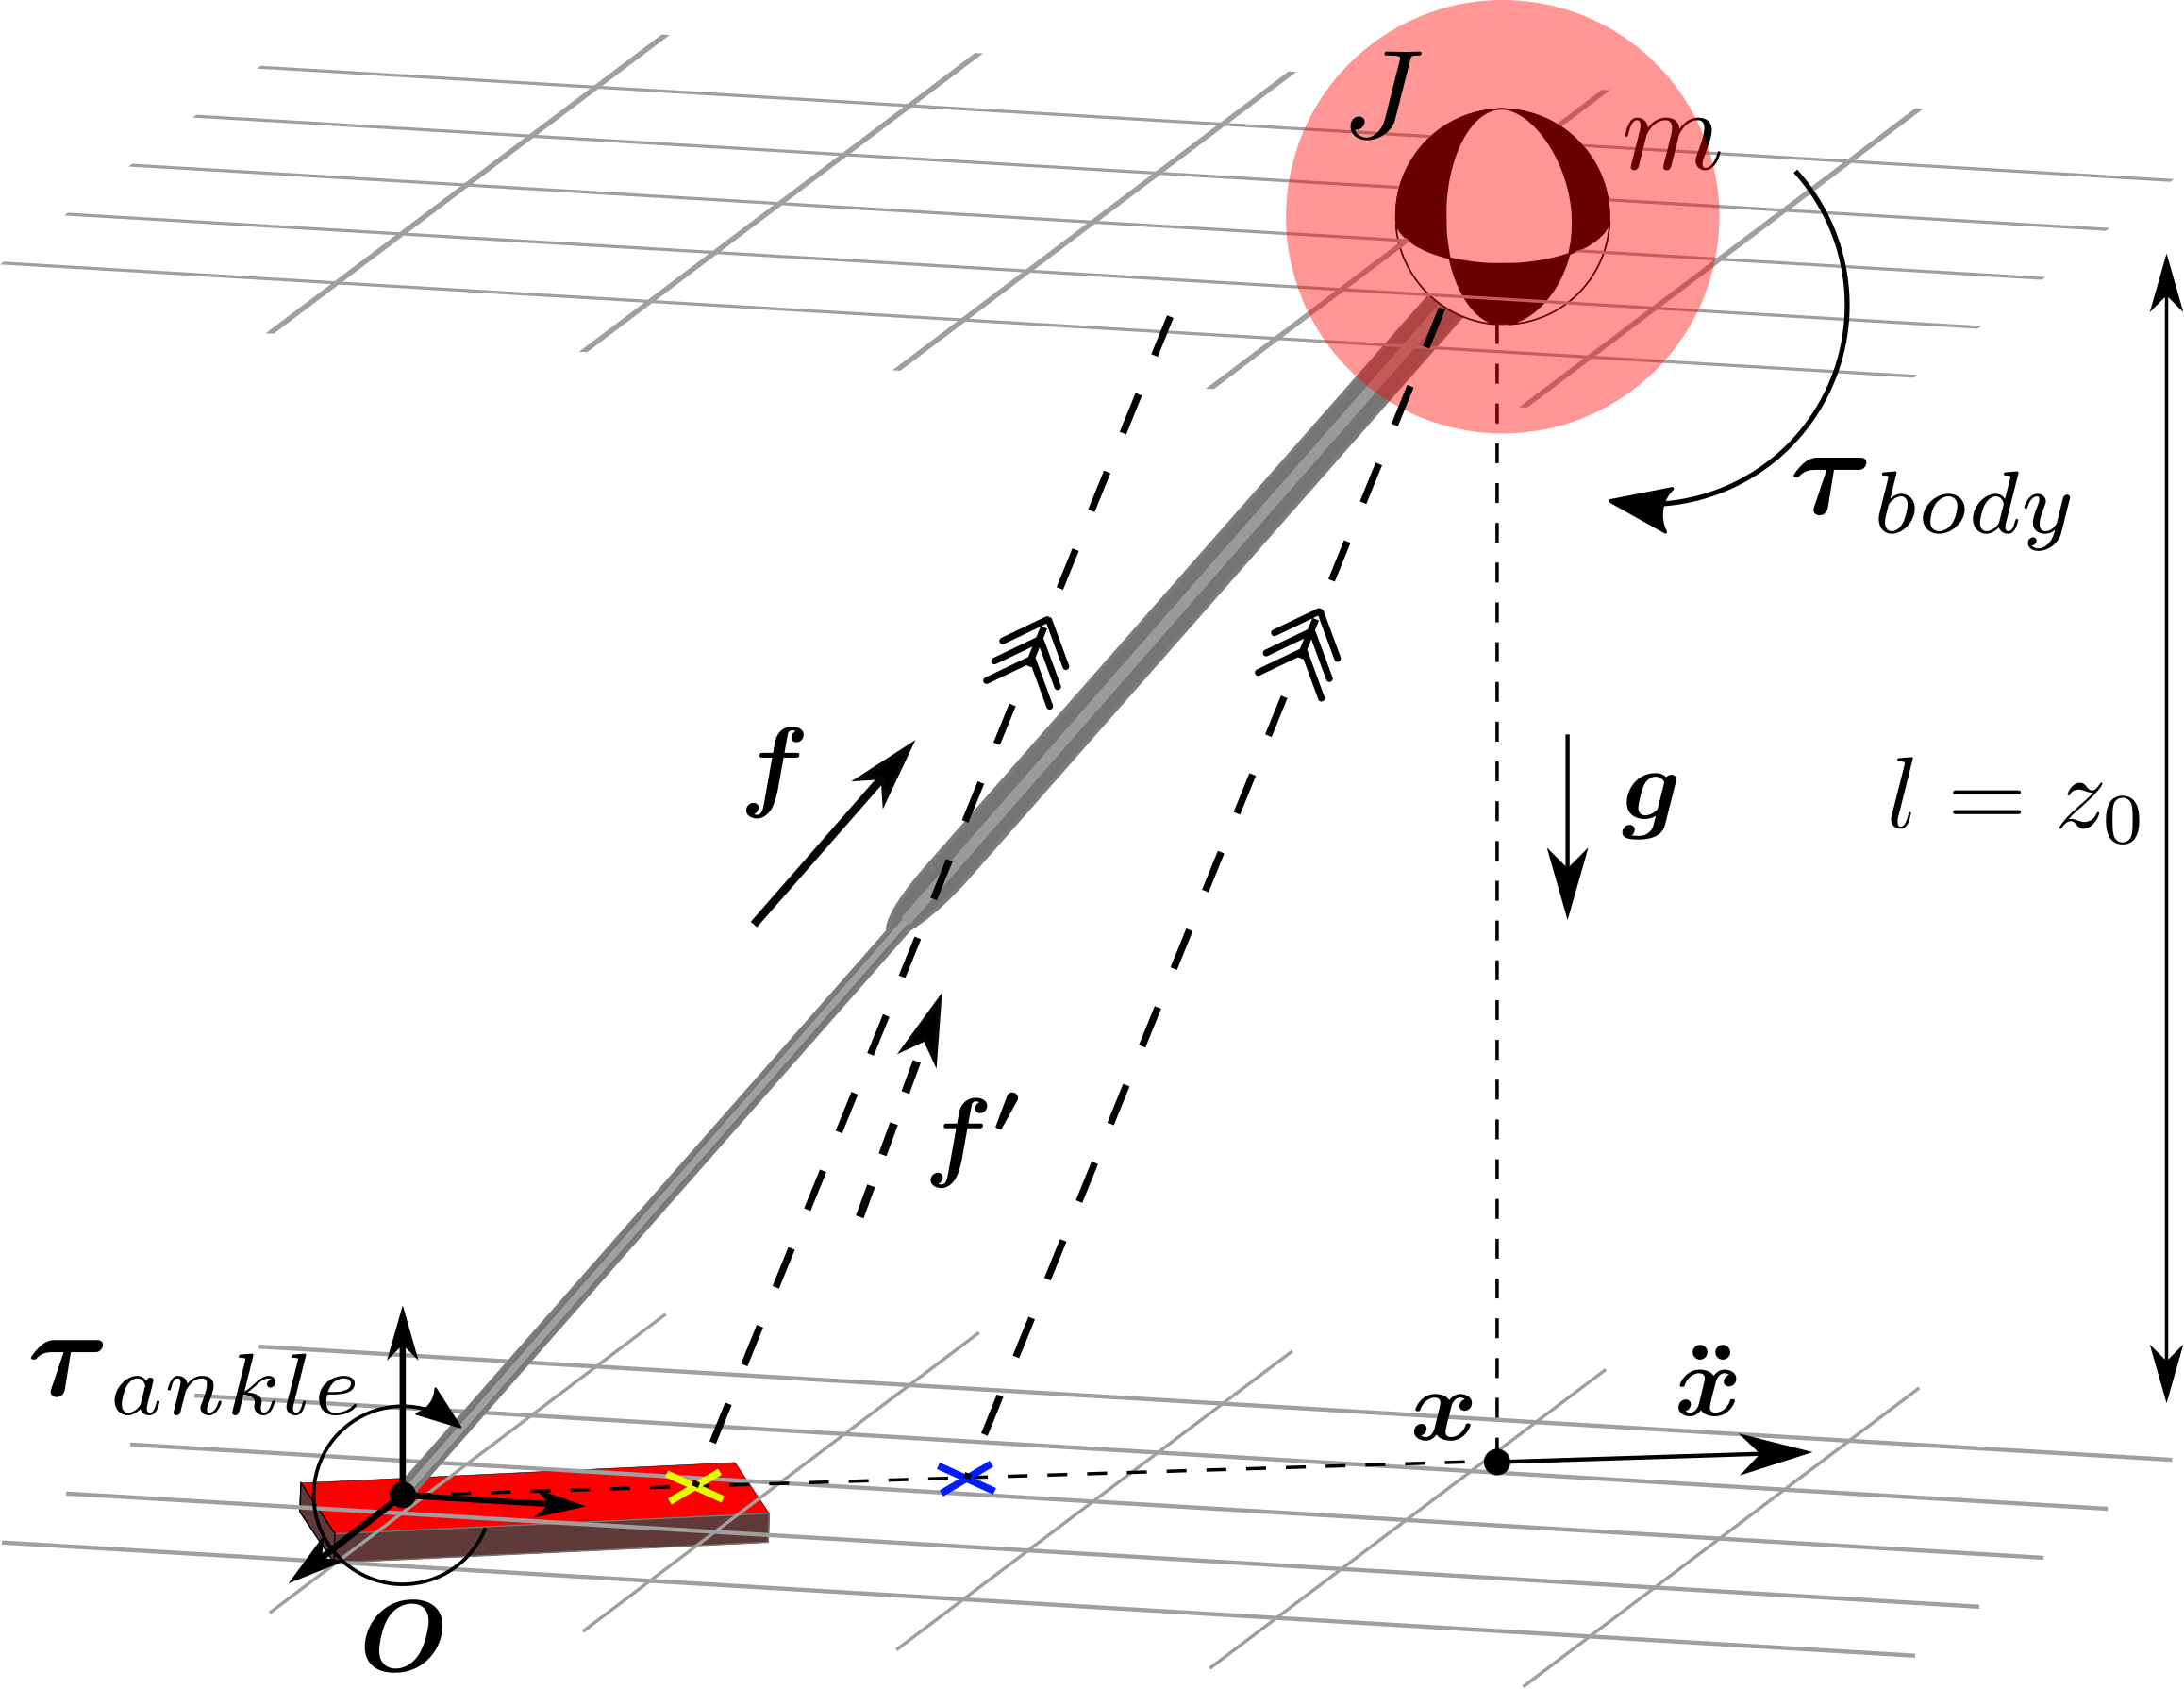
\includegraphics[width=0.5\textwidth]{STYLESTUFF/3DCoMwithfootinertia.png}
\caption{\ac{3D} motion of \ac{LIP} model with foot}
\label{fig:3dlipfoot}
\end{figure}
\subsection{Other points}
\ac{eCMP} \ac{VRP}
\section{Planning}
For control of a robot, first a motion plan has to be generated. As the dynamics of a humanoid robot are very complex and underactuated, there exist numerous ways to do this. 
\subsection{Footstep planning}
While not all bipedal robots require a footstep plan to walk, most humanoids do. A footstep plan is a sequence of foothold references on the ground, which can be computed either offline, online or offline with online adjustment. There are various ways how this can be done, but as this can be entirely uncoupled of the research area of focus in this report this is not further discussed. The footstep plan is assumed to be given beforehand. [REF REF]

\subsection{Trajectory planning}
Again, there are numerous ways to plan the body path of a humanoid. There are differences in planning in joint-space and planning only a \ac{CoM} trajectory for example. This is greatly depending on the control strategy that is used. Currently at IHMC a \ac{ICP} plan is generated based on a footstep plan with \ac{CoP} knot points. Based on the desired time of the footstep plan, the \ac{ICP} dynamics are integrated backwards in time to come to a reference trajectory. This plan is than tracked using PD-control, where the \ac{CoP} and angular momentum are used as control inputs. 

\subsection{Swing Leg trajectories}
If the robot places its foot from the current footstep to the next, a more local plan is generated. This is often done by defining a polynomial spline from the one foothold to the other, with knot points at a certain height above the ground to make the foot not hit the ground. This spline is generated as a set of piece-wise minimum jerk trajectories. The minimum jerk trajectory minimizes the jerk, the third derivative of position with respect to time, and needs a desired completion time for the trajectory as input. This desired time for the entire spline is called the desired Swing Time for this step. 

\section{Control}
To track a generated plan the system has to be controlled. PD-control, LQR and MPC are all used in humanoid robotics. Again, there are differences in joint-level control and for example the control of the desired \ac{CoM} position, which often are separated in high level and low level control. In some cases, like with the \ac{HZD} approach as described in \cite{westervelt2003hybrid}, there is no decoupling in such levels. However, the \ac{HZD} is for this reason often applied to simpler robots, as in the paper and on ATRIAS. Furthermore, the \ac{HZD} approach is designed for system with a degree of underactuation of one, which corresponds more to a \ac{2D} than a \ac{3D} robot model. 
\subsection{High level control}
Tracking the \ac{ICP} trajectory as is done at IHMC is an example of high level control. The robot in this stage can be seen as an \ac{LIP} with a finite sized foot and body angular momentum. At a current footstep, using the right combination of ankle torque and angular momentum, the robots motion can be controlled. The robot is assumed to keep itself at a constant height and expected to generate the desired angular momentum. 
\subsection{Low level control}
As the real robot is not a \ac{LIP} and cannot generate high level control inputs as angular momentum as a single control input, a second layer of control is needed: joint or low level control. Low level controllers are often based on inverse kinematics and inverse dynamics. This is concept also widely used in industrial robotic manipulators. One of the main difficulties with low level control is compliance.
\subsection{Compliant control}
In the walking of a bipedal robot with legs hybrid switching between Swing and Stance phase, a problem gets introduced with this hybrid phase shift. During Swing, a trajectory is tracked using position based control. When the foot hits the ground, it switches instantly to the Stance Phase, where its position is fixed and its control actions are mainly based on forces. This causes instant switch can cause instabilities and an agile, compliant control strategy is needed. Low level controllers are often based on complex whole-body controllers, which can generate configurations and angular momenta upon request of the higher level commands. Due to compliant capabilities, the full joint space control commands are often outputs of an optimization program.   

\section{Varying CoM Height Planning and Control}
As mentioned earlier, the recently work has been done in keeping the constant height assumption away from the walking model. The motivation for this is twofold. The use of height can be used in tracking control. Where angular momentum and \ac{CoP} are the two control inputs for a \ac{LIP} model, the use of height, thus a varying leg force, can be used as a third input. Furthermore, in motion over un-flat terrain a varying height model can give a better approximation of how the dynamics will behave over time. In other word: planning can be improved. 
\subsection{\ac{DCM} for varying height}
One attempt to use a varying height model for planning is the introduction of the \ac{DCM} in \cite{englsberger2013three}. This is used in a rough terrain planning model. The \ac{DCM} is defined as
\begin{equation}
\boldsymbol{\xi} = \boldsymbol{x} + b\boldsymbol{\dot{x}}
\end{equation}
where $\boldsymbol{\xi}=[\xi_x,\xi_y,\xi_z]^T$ is the \ac{DCM}, $\boldsymbol{x}=[x_{CoM}, y_{CoM}, z_{CoM}]^T$ and $\boldsymbol{\dot{x}}=[\dot{x}_{CoM}, \dot{y}_{CoM}, \dot{z}_{CoM}]^T$ are the \ac{CoM} position and velocity and $b>0$ is the time-constant of the \ac{DCM} dynamics. 
[ZOEK UIT HOE VRP EN ECMP VERKREGEN ZIJN].
\cite{hopkins2014humanoid} defines the constant $b=1/\omega_0$, where $\omega_0=\sqrt{\frac{g}{z_{CoM}}}$. This makes it the same as the \ac{ICP}, but with a $z$ component in the state. The \ac{DCM} is derived with respect to time, where $\omega$ is posed to be time varying, so the height is time varying. This brings a new expression for the so called \ac{DCM}.
\cite{caron2018capturability} uses the \ac{DCM} for a MPC control scheme to capture the inverted pendulum \ac{CoM}.

\subsection{Orbital Energy for nonlinear \ac{CoM} trajectories}
The true non-linear model of a traveling \ac{CoM} subject to a force coming from the $[0,0]$ point on the ground is for the \ac{2D} $xz$\nobreakdash-plane
\begin{eqnarray}
m\ddot{x} = F \frac{x}{\sqrt{x^2+z^2}}\\
m\ddot{z} = -mg+F \frac{z}{\sqrt{x^2+z^2}}
\label{eq:nonlindyn}
\end{eqnarray} 
where $F$ is the ground reaction force. \cite{pratt2007derivation} constrains $z=f(x)$ and integrates  the equations of motion over time, how a similar conservation of Orbital Energy as in Eq. \eqref{eq:Elip} is derived. This Orbital Energy however is not based on a straight line, but depends on the function $f(x)$. The  full integration can be found in the paper, but the final expression writes as
\begin{equation}
    \frac{1}{2}\dot{x}^2\bar{f}^2(x)+gx^2f(x) - 3g\int_{x_0}^xf(\xi)\xi d\xi = \frac{1}{2}\dot{x}_0^2\bar{f}^2(x_0)+gx_0^2f(x_0).
\end{equation}
where $\bar{f}(x)=f(x)-f'(x)x$, $[x_0,\dot{x}_0]$ is the initial horizontal state and velocity and $[x,\dot{x}]$ is the current horizontal state and velocity. There is experimented in simulation with a symmetric polynomial, where the trajectory is tracked using a PD feedback scheme where the leg force is the control input. The polynomial description makes the integral directly solvable. To make a clear seperation between \ac{Elip}, this energy form will be defined later as \ac{Eorbit}.\\
Recently, this is used in a \ac{MPC} formulation and basic simulations have been done by \cite{koolen2016balance}. The main idea in this paper is to define four constraints on the trajectory $f(x)$, which define the four constants of a cubic polynomial by a matrix inversion. Those consist of two constraints on the initial conditions, one constraint on the final condition and one constraint on the Orbital Energy conservation. The matrix inversion is done offline, so that the control input can directly be written as a function of the polynomial constants and thus of the initial and final states. 

\subsection{Other varying height approaches}
Besides derivations of the \ac{ICP} for varying height and the \ac{Eorbit}, there are other approaches that describe the effects of varying height. The authors of \cite{gao2017increase} come up with different strategies to use varying height to generate impact or to relatively speed up the \ac{CoM} motion compared to the \ac{ICP} trajectory. Besides gravity, an extra vertical acceleration constant is added in the \ac{LIP} equations of motion. \\
An applied approach is described in \cite{nguyen2017dynamic}. For different step lengths and step heights, trajectories are generated offline using a direct collocation optimization framework. Online is interpolated between trajectories with knowledge of the current step and the upcoming step. The trajectories are on joint level and make use of the earlier discussed \ac{HZD} approach. This is applied on hardware, but with the sagittal motion supported and thus only the \ac{2D} dynamics in the $xz$-plane are considered.

\subsection{Trajectory optimization for nonlinear systems}
As becomes clear, looking at the simplified varying height robot model, nonlinearity is the main bottleneck. As such, it would be rewarding to have already an insight in trajectory optimization for such systems. \cite{kelly2017introduction} poses a MATLAB  toolbox that can be used to solve trajectory optimization problems. Furthermore, it gives a lot of information how the solvers work. The methods distinguish themselves between direct and indirect methods, shooting and collocation methods and the difference between the so called \'h'- and \'p'-methods. The latter two define the degree of segmentation and the order of used functions between the segments of the problem. Direct collocation methods are most likely best suited for the subject of interest, as they require less computation time than indirect and shooting methods. Using the system description of Eq. \eqref{eq:nonlindyn}, a direct collocation method could be used for generating a capture trajectory for example. 




